Durante el año de realización de este trabajo para la cátedra de Proyecto Final, se realizó una serie de análisis orientados a la gestión, previsión y orden del proyecto.
En esta sección se muestran los análisis específicos que formaron parte de la gestión del proyecto.



\subsection{Gestión del tiempo}
\label{sec:tiempo}
{\centering
	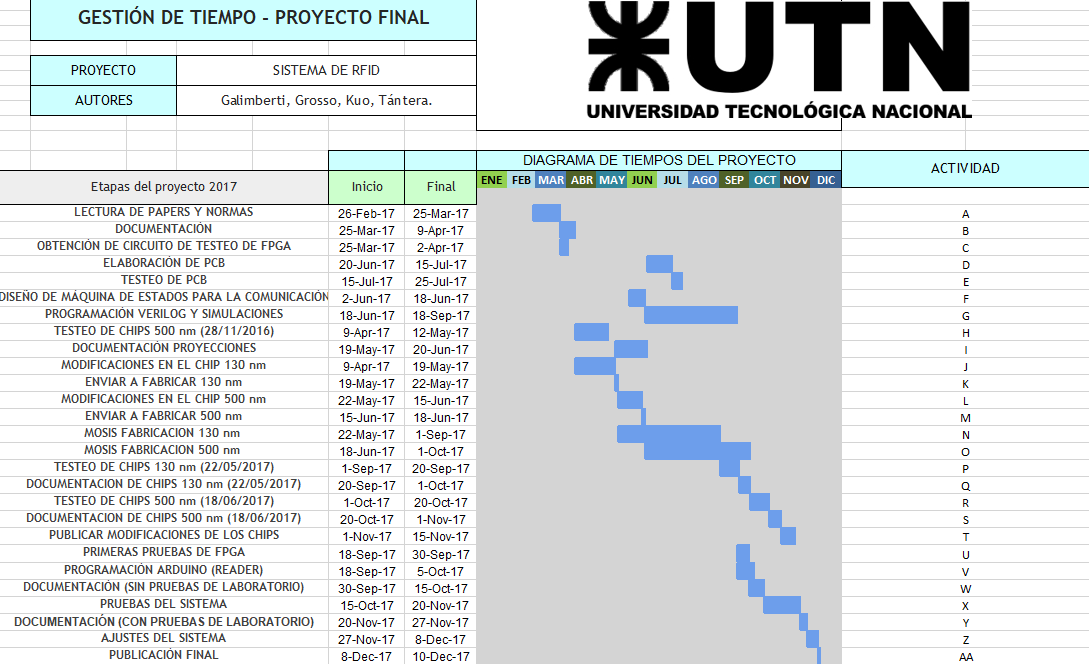
\includegraphics[scale=0.55]{Gestion/GDT.png}
}
\newline
\newline

\label{sec:tiempo}
{\centering
    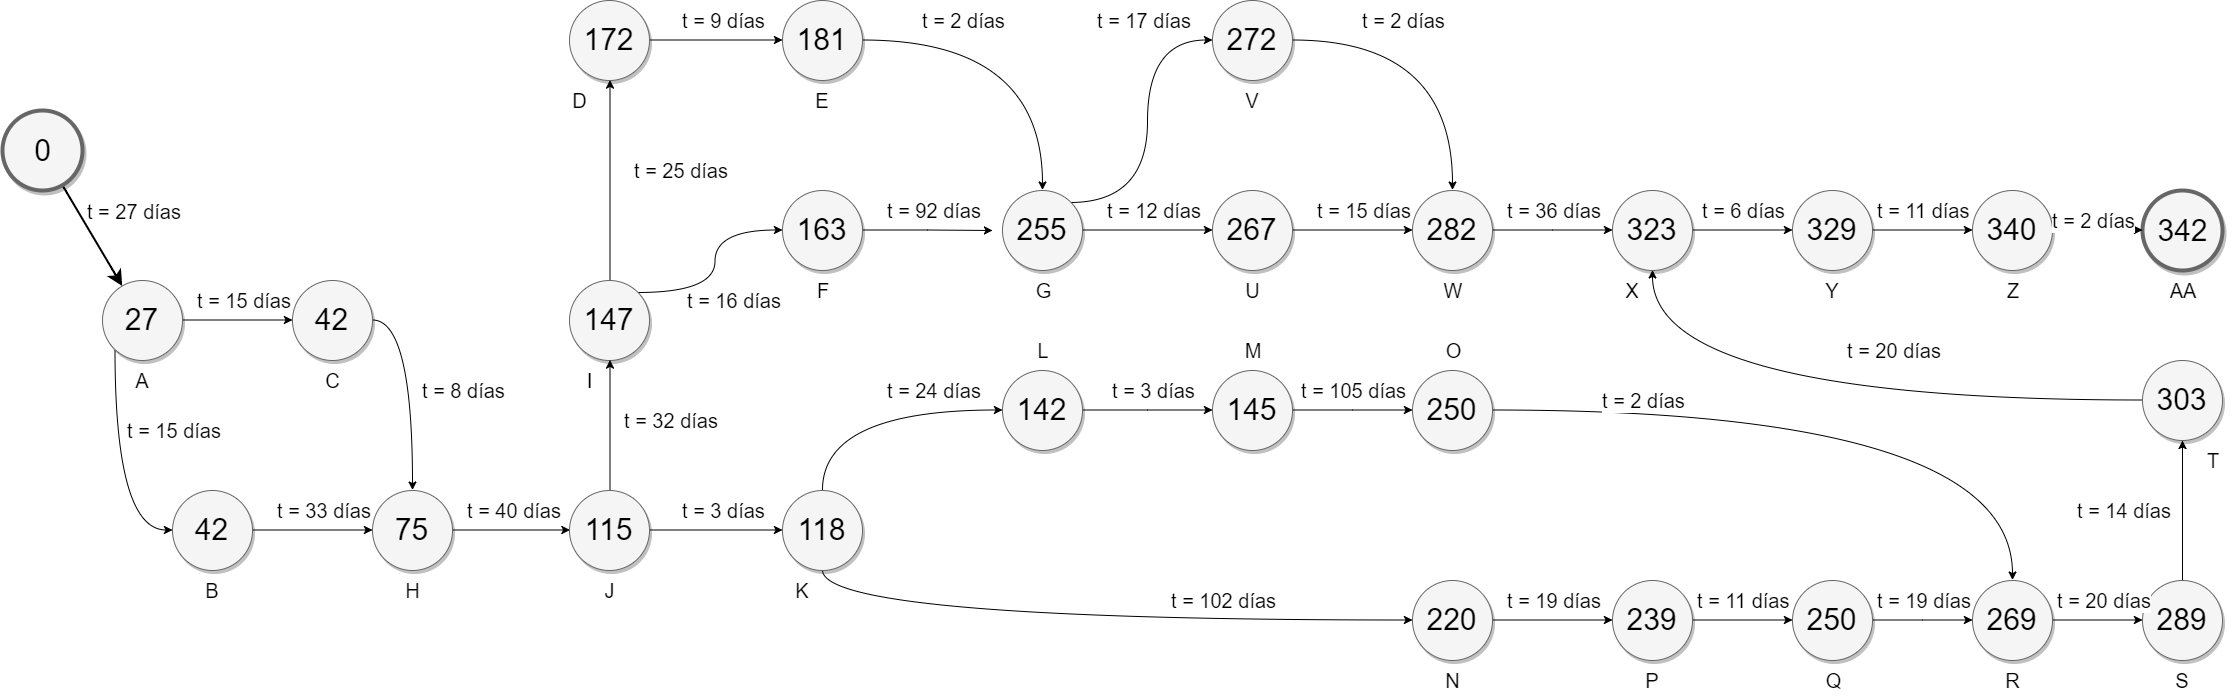
\includegraphics[scale=0.2]{Gestion/diagrama_de_tiempo.png}
}
\newpage
\subsection{Matriz FODA}
\label{sec:FODA}
Analizando el proyecto y las situaciones externas a éste, se procedió al armado de la matriz que refleja: \newline 
- Fortalezas y debilidades internas \newline  
- Oportunidades y amenazas externas \newline
{\centering
	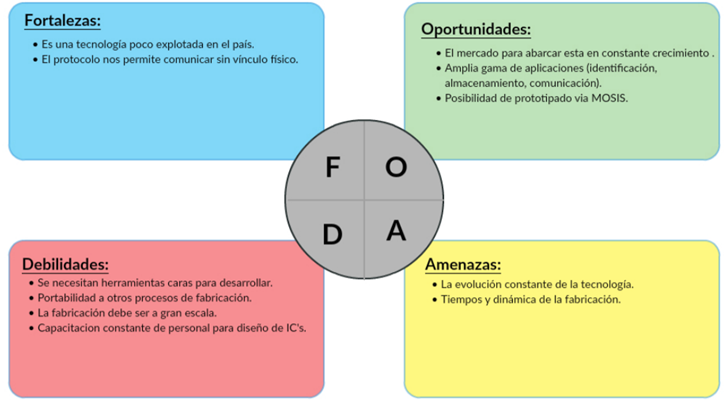
\includegraphics[scale=0.8]{Gestion/FODA.png}
}


\subsection{Gestión de problemas}
\label{sec:problemas}
Como principales problemas podemos detectar 3
\begin{enumerate}
\item No disponer del chip:
	\begin{itemize}
    	\item Dada de baja a la tecnología en la cual se realizó el desarrollo.
		\item Debido a discontinuidad de las corridas por aprte de las foundries (On Semi Conductors 500nm o Global Foundries 130nm).
		\item Debido a retrasos en la entrega de las foundires.
	\end{itemize}
\item No poder realizar modificaciones en el chip:
    \begin{itemize}
    	\item Inconvenientes en el desarrollo y empleo de PDK's.
		\item Que surjan inconvenientes con el uso de las licencias o no poseerlas.
    \end{itemize}
\item Mal funcionamiento del chip
	\begin{itemize}
        \item Dispersiones fuera de rango en la fabricación del mismo. 
	\end{itemize}
\end{enumerate}

\newpage

\subsection{Gestión de objetivos}
\label{sec:objetivos}
En función de los inconvenientes comentados en la gestión de problemas se plantean los siguientes objetivos
\begin{enumerate}
\item Abstracción de variabilidades en foundries:
	\begin{itemize}
    	\item Migración de tecnología (por ejemplo de 500nm a 130nm).
		\item Realizar la corrida actual en varias tecnologías para asegurar una entrega.
		\item Disponibilidad del circuito en discreto.
	\end{itemize}
\item Uso de herramientas confiables:
    \begin{itemize}
    	\item Utilizar los PDK's nativos otorgados por las foundries.
		\item Poseer confiabilidad en el servidor y una correcta configuración del mismo.
    \end{itemize}
\item Disminuir la probabilidad de errores en la fabricación del chip:
	\begin{itemize}
        \item Simulación con corners y metodología "Montecarlo". 
	\end{itemize}
\end{enumerate}

\subsection{Matriz de riesgos}
\label{sec:riesgos}
Análisis del nivel de riesgo de las tareas sobre la realización del proyecto.


\begin{tabular}{|l|r|r|r|r|r|}
\hline \multirow{2}{1.8cm}{PROBABIL.}
& \multicolumn{5}{p{10cm}|}%
{\centering IMPACTO}\tabularnewline \cline{2-6}
& \multicolumn{1}{p{1.7cm}|}%
{\centering MUY BAJO}
& \multicolumn{1}{p{1.7cm}|}%
{\centering BAJO}
& \multicolumn{1}{p{1.7cm}|}%
{\centering MEDIO}
& \multicolumn{1}{p{1.7cm}|}%
{\centering ALTO}
& \multicolumn{1}{p{1.7cm}|}%
{\centering MUY ALTO}

\tabularnewline \hline
MUY ALTA &\cellcolor{yellow}&\cellcolor{orange}&\cellcolor{orange}Interrupción de trabajo&
\cellcolor{red}&\cellcolor{red}\\
&\cellcolor{yellow}&\cellcolor{orange}
&\cellcolor{orange}debido a exámenes&
\cellcolor{red}&\cellcolor{red}\\
\hline
ALTA&\cellcolor{green}
&\cellcolor{yellow}
&\cellcolor{orange}
&\cellcolor{orange}&\cellcolor{red} \\
&\cellcolor{green}&\cellcolor{yellow}
&\cellcolor{orange}&
\cellcolor{orange}&\cellcolor{red}\\   
\hline
MEDIA&\cellcolor{green}&\cellcolor{yellow}Falta de stock
&\cellcolor{yellow}Malfuncionamiento&
\cellcolor{orange}Atraso en entrega de&\cellcolor{orange}Falla de la\\
&\cellcolor{green}&\cellcolor{yellow}de componentes
&\cellcolor{yellow}de placa de test&
\cellcolor{orange}chip&\cellcolor{orange}fabricación \\
\hline
BAJA   &\cellcolor{green}
&\cellcolor{green}Demora en la
&\cellcolor{yellow}Falta de &
\cellcolor{yellow}Malfuncionamiento&\cellcolor{orange} Mal diseño\\
&\cellcolor{green}
&\cellcolor{green}fabric. de placa
&\cellcolor{yellow}documentacion&
\cellcolor{yellow}de FPGA&\cellcolor{orange}del chip\\
\hline
 MUY BAJA   &\cellcolor{green}&\cellcolor{green}&\cellcolor{green}&
 \cellcolor{green}Malfuncionamiento&\cellcolor{yellow}No disponibilidad\\
 &\cellcolor{green}&\cellcolor{green}&\cellcolor{green}
 &\cellcolor{green}de arduino (reader)&\cellcolor{yellow}de herramienta\\
\hline
\end{tabular}



\newpage
\subsection{KPI's}
\label{sec:descripción}
A continuación enunciaremos cómo se conformaron nuestros indicadores y en que valor se encuentran actualmente
\begin{itemize}
\item Hitos Fallidos (HF): Mide el porcentaje de hitos fallidos a tiempo sobre el total de hitos.
	\begin{itemize}
    	\item Tendencia deseada: Negativa.
		\item Periodo de captura: Mes.
		\item Frecuencia de medida: mensual.
	\end{itemize}
\item Retraso del proytecto (RP): Mide el retraso total del proyecto mediante la suma de los retrasos registrados en cada uno de los estados de implementación del proyecto.
	\begin{itemize}
    	\item Tendencia deseada: Negativa.
		\item Periodo de captura: Ejercicio hasta la fecha.
		\item Frecuencia de medida: Mensual.
	\end{itemize}
\item Tareas Atrasadas (TA): Mide el porcenta de tareas retrasadas del número total de tareas actuales.
	\begin{itemize}
    	\item Tendencia deseada: Negativa.
		\item Periodo de captura: Puntual.
		\item Frecuencia de medida: Semanal.
	\end{itemize}
\item Incidencias Identificadas en el Proyecto (IIP): Mide el número de nuevas incidencias que son identificados y necesitan resolverse una vez iniciado el proyecto.
	\begin{itemize}
    	\item Tendencia deseada: Negativa.
		\item Periodo de captura: Semanal.
		\item Frecuencia de medida: Semanal.
	\end{itemize}
\item Riesgos (R): Mide el número de riesgos identificados.
	\begin{itemize}
    	\item Tendencia deseada: Positiva.
		\item Periodo de captura: Puntual.
		\item Frecuencia de medida: Trimestral.
	\end{itemize}
\item Riesgos Posibles (RPo): Mide el porcentaje de riesgos que todavía pueden tener lugar en el momento del proyecto.
	\begin{itemize}
    	\item Tendencia deseada: Negativa.
		\item Periodo de captura: Puntual.
		\item Frecuencia de medida: Mensual.
	\end{itemize}
\item Plazos de Entrega Cumplidos (PEC): Mide el porcentaje de plazos de entrega cumplidos durante el proyecto sobre el total.
	\begin{itemize}
    	\item Tendencia deseada: Negativa.
		\item Periodo de captura: Puntual.
		\item Frecuencia de medida: Mensual.
	\end{itemize}
\end{itemize}

Algunos de los valores que tomaron los KPI's durante el proyecto fueron los siguientes:

\begin{center}
  \begin{tabular}{ | l | c | l |}
    \hline
    KPI & Valor & Detalle \\ \hline
    HF & 3.84\% & Retraso en la finalización del PCB sobre un total de 26 hitos.\\ \hline
    RP & 0.5 &  Medio mes de retraso en la finalización del PCB.\\ \hline
    TA & 14.28\% & Una sola tarea en un total de nueve activas. \\ \hline
	IIP & 1  & Incompatibilidad con ISE. \\ \hline
	R & 2  & Dos de los tres riesgos están latentes al momento, no disponer ni poder modificar el chip.\\ \hline
	RPo & 100\% & Todos los riesgos pueden tener lugar. \\  \hline
    PEC & 94.4\% & Diecisiete de los dieciocho plazos de entrega fueron cumplidos. \\
    \hline
  \end{tabular}
\end{center}


